\section{System}
Das Projekt kann in drei Systeme unterteilt werden. Das vorhandene System von Varian ist das erste. Das zweite System ist eine Zwischenlösung, um mit der Entwicklung der Firmware anzufangen, ohne das die eigene Hardware schon vorhanden ist. Und dass dritte System ist das endgültige System, welches das System von Varian emuliert.

\subsection{System Varian}
\begin{figure}[tb]
    \centering
    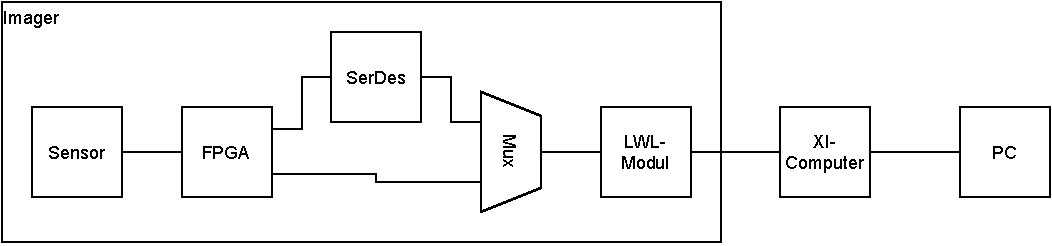
\includegraphics[width=\linewidth]{bd_varian}
    \caption{Blockdiagramm des Systems von Varian}
    \label{fig:bd_varian}
\end{figure}

Das System der Varian besteht aus dem Imager und dem XI-Computer. Wobei diese beiden Blöcke Teil eines Röntgengerätes für medizinische Zwecke sind. Der Imager ist ein Bildsensor für Röntgenstrahlen und sendet die gemessenen Bilder über eine LWL-Schnittstelle zum XI-Computer. Der XI-Computer empfängt die Bilder und lässt diverse Algorithmen darüber laufen. Unter anderem auch Algorithmen zur Erkennung von Pixelfehlern. Das mit den Algorithmen bearbeitete Bild wird wiederum über Ethernet an einen externen Computer gesendet.

Um die Bilder vom Sensor auszulesen, zu digitalisieren und zu übertragen, sitzt auf dem Imager ein FPGA. Dieser sendet die Bilder zum XI-Computer ent\-weder über einen vom FPGA internen oder externen Serialisierer/Deserialisierer, kurz SerDes, zu einem LWL-Modul. Der FPGA kommuniziert über einen parallelen Bus mit dem externen SerDes. Die beiden SerDes senden ein LVDS Signal zum LWL-Modul. Das LWL-Modul ist ein standardisiertes Small Form-factor Pluggable (SFP). Um zwischen den beiden SerDes auszuwählen, gehen die Tx-Signale auf einen Multiplexer und die Rx-Signale auf einen Demultiplexer, dieser wird der Einfachheitshalber nur Mux genannt. Das beschriebene System ist im Blockschaltbild in Figure \ref{fig:bd_varian} zu sehen.

Der Vorteil des internen SerDes ist die Geschwindigkeit. Der externe SerDes kann Daten mit einer Übertragungsrate von 1.25Gbps übertragen und der interne mit 6Gbps. Die älteren Versionen des Imagers arbeiten nur mit dem externen SerDes und die neueren mit beiden. Da stellt sich die Frage, wieso überhaupt den externe SerDes brauchen? Beim Einschalten des Imagers ist der FPGA noch nicht konfiguriert und solange der FPGA nicht konfiguriert ist, ist auch der interne SerDes nicht konfiguriert. Somit braucht es den externen SerDes, um vom XI-Computer aus den FPGA zu konfigurieren. Sobald der FPGA konfiguriert ist, schaltet dieser auf den internen SerDes um und kommuniziert mit dem XI-Computer über diesen. Welche SerDes die verschiedenen Versionen des Imagers besitzen ist in Tabelle \ref{tab:sensorVersionen} ersichtlich.

\begin{table}[tb]
    \centering
    \caption{Eckdaten der verschiedenen Sensorversionen der Varian}
    \begin{tabular}{|l|l|l|l|l|}
        \hline
        \textbf{Imager} & \textbf{Auflösung} & \textbf{Pattern}$^1$ & \textbf{FPGA} & \textbf{Schnittstelle} \\
        \hline
        DMI$^2$ & 1280x1280 & \pbox[t]{10cm}{b10’1010’1010’1010’1010\\XI: 0xAAA\vphantom{)}} & \pbox[t]{10cm}{Spartan 3\\XC3S200} & externer SerDes\\
        \hline
        \pbox[t]{10cm}{RTI 1.0$^2$\\(RTI4343L)} & 1280x1280 & \pbox[t]{10cm}{b10’1010’1010’1010’1010\\XI: 0xAAA} & \pbox[t]{10cm}{Spartan 3\\XC3S200} & externer SerDes\\
        \hline
        \pbox[t]{10cm}{RTI 2.0\\(RTI4343iL)} & 3072x3072 &\pbox[t]{10cm}{b10’1010’1001’0101’0101\\XI: 0x955} & \pbox[t]{10cm}{Artix 7\\XC7A100T} & \pbox[t]{10cm}{aktuell:\\externer Serdes\\zukünftig:\\MGT(GTP)} \\
        \hline
        \pbox[t]{10cm}{RTIXL 1.0\\(RTI8643L)} & 6144x3072 & \pbox[t]{10cm}{b10’1010’1001’1001’0101\\XI: 0x995} & \pbox[t]{10cm}{Artix 7\\XC7A200T} & \pbox[t]{10cm}{externer SerDes\\und MGT(GTP)}\\
        \hline
       \end{tabular}
       \begin{tabular}{l}
        {\footnotesize $^1$}\pbox[t]{0.9\linewidth}{\footnotesize Das XI wertet nur die letzten 12 bit des Pattern aus. Um das DC-Balancing zu erreichen, müssen trotz\-dem alle 18 bits korrekt gesendet werden.}
        \\
        {\footnotesize$^2$}\pbox[t]{0.9\linewidth}{\footnotesize DMI und RTI 1.0 besitzen exakt die gleiche Elektronik.}

       \end{tabular}
    \label{tab:sensorVersionen}
    \end{table}

\subsubsection*{Bootvorgang}
\label{sec:varian_boot_sequence}
Das Bitfile um den FPGA zu konfigurieren wird bei jedem Start vom XI-Computer über den externen SerDes auf den FPGA geladen. Dazu müssen sich zuerst die beiden SerDes, also der auf dem Imager und der auf im XI-Computer, synchronisieren. Damit der XI-Computer weiss, welcher FPGA auf dem Imager vorhanden ist, liegt ein Bitmuster mittels Pull-Up und Pull-Down Widerständen an den Tx-Leitungen des SerDes auf dem Imager. Somit ergibt sich folgende Bootsequenz.

Zuerst aktiviert der XI-Computer den Sync-Eingang seines SerDes. Somit kann sich der Rx-Pfad des SerDes auf dem Imager mit dem Tx-Takt des SerDes auf dem XI-Computer synchronisieren. Um dies zu erreichen sendet der SerDes ein Sync-Muster. Der Sync-Eingang des SerDes auf Imagers ist auf einen Rx-Kanal von sich selber angeschlossen. Somit kann der XI-Computer den SerDes auf dem Imager in den Sync-Modus versetzen. Dieser wird, sobald das Rx-Pfade des SerDes auf dem Imager synchronisiert ist, aktiviert. Nun sind beide Pfade der SerDes synchronisiert.

Als nächstes liest der XI-Computer das Versionmuster auf dem Imager aus. Aufgrund von diesem konfiguriert er den FPGA auf dem Imager mit dem entsprechenden Bitfile. Nun ist der FPGA konfiguriert und der Imager kann auf die Befehle vom XI-Computer reagieren. 

\subsubsection*{Kommunikation zwischen Imager und XI-Computer}
\label{sec:varian_com}

Man kann zwischen dem XI-Computer und dem Imager von einer Master-Slave Beziehung reden. Der XI-Computer hat die Möglichkeit dem Imager verschiedene Befehle zu senden, welche der Imager daraufhin ausführt. Es gibt drei verschiedene Gruppen von Befehlen. Es gibt die Write-Befehle, welche dem Imager Einstellungen übermitteln, die der Imager in einem Register speichert. Mit den Read-Befehlen kann der XI-Computer diese Einstellungsregister wieder auslesen. Und als letztes gibt es noch den Trigger-Befehl. Die Write-Befehle beinhalten eine Adresse und einen Wert, die Read-Befehle nur eine Adresse. Mit dem Trigger-Befehl kann der XI-Computer ein Bild anfordern. Ein Trigger-Befehl hat Vorrang vor Write- und Read-Befehlen. Die genaue Auflistung aller Einstellungsregister und deren Aufgabe kann in der Dokumentation des Imagers entnommen werden. \cite{varian}

Der FPGA liest immer Zeile für Zeile die Werte des Sensors aus. Solange kein Trigger-Befehl vom XI-Computer gesendet wird, werden die Zeilen verworfen. Sobald ein Trigger-Befehl kommt, wartet der FPGA bis er die letzte Zeile ausgelesen hat und verwirft auch diese noch. Wenn der FPGA nun wieder bei der ersten Zeile angelangt, fängt er an das Bild Pixel für Pixel, Zeile für Zeile zu übertragen. Am Anfang des Bildes vor der ersten Zeile sendet der FPGA ein \textit{Frame-Start} Signal. Und vor jeder Zeile überträgt er ein \textit{Line-Start} Signal. Vor der ersten Zeile muss kein zusätzliches \textit{Line-Start} Signal gesendet werden. Pro Takt wird ein Pixel übertragen. Der FPGA überträgt eine Zeile erst wenn er sie vollständig vom Sensor ausgelesen hat. Dafür überträgt er die Zeile Pixel für Pixel ohne Unterbruch. Ein Pixel ist 16 Bit gross und somit genau gleich gross, wie die parallele Schnittstelle zum SerDes. Um immer eine Zeile vom Sensor auszulesen und eine Zeile zu übertragen speichert ein dual-port RAM die Pixelwerte.

Die Read-Befehle werden nur ausgeführt, wenn keine Bilddaten zu senden sind. Daher werden sie in einem Fifo zwischengespeichert und bei Möglichkeit übertragen. Die Read-Befehle dürfen nur zwischen Zeilen oder Bildern übertragen werden und nicht zwischen einzelnen Pixeln. Da es länger dauert eine Zeile von Sensor zu lesen, als eine Zeile an den XI-Computer zu senden, bleibt immer etwas Zeit um die Read-Befehle vom Fifo abzuarbeiten. Wie vor einem neuen Bild und einer neuen Zeile gibt es das \textit{Command} Signal, dieses wird immer vor der Antwort auf einen Read-Befehls gesendet. Die Antwort eines Read-Befehls bestehen aus den Daten aus dem Einstellungsregister und der entsprechenden Adresse.

\subsubsection*{Wahl des FPGAs}
Das oben beschriebene System der Varian soll emuliert werden. Die Vorgabe ist es 100 Bilder speichern zu können. Mit einer maximalen Bildgrösse von 6144x3072x16 ergibt dies etwa 3.5GB Daten. Als Recheneinheit ist die Vorgabe einen FPGA von Xilinx zu nehmen. Dies ist vom Auftragsgeber, Varian, vorgegeben, da sie mit diesen FPGAs arbeiten und wir somit auch vorhandenen Code für die LWL-Schnittstelle übernehmen können. Die Daten sollen via USB auf das Gerät geladen werden und über die LWL-Schnittstelle weiter zum XI-Computer. Daher braucht das System eine Hardware für das USB und eine für die LWL-Schnittstelle. Für das USB kommt entweder ein externer Chip infrage oder der FPGA muss ein integriertes USB-Modul besitzen. Die LWL-Schnittstell der Varian ist nicht vollständig standardisiert, daher muss diese mit externen Bauteilen aufgebaut werden. Der interne SerDes ist ein Multi-Gigabit-Transiever (MGT). Die FPGAs von Xilinx haben verschiedene MGTs, welche nicht alle die nötigen Geschwindigkeit unterstützen. \cite{mgt} Das Schema der LWL-Schnittstelle kann von der Varian übernommen werden. Um Übertragungsgeschwindigkeiten bis 6GBps zu unterstützen, muss der Speicher und der FPGA über eine entsprechend schnelle Schnittstelle kommunizieren können. Da das Layouten einer solchen Schnittstellen eine komplexe Angelegenheit ist und bei der Inbetriebnahme zusätzliche Tests benötigt, haben wir uns entschieden ein FPGA-Modul zu verwenden, auf welchem der Speicher schon vorhanden ist. 

Mit diesen Anforderungen haben wir fünf verschiedene Varianten von den Firmen Enclustra und Trenz-Electronic gefunden. Da FPGA-Module mit 4GB RAM sehr teuer sind, haben nicht alle die Kapazität 100 Bilder bei voller Auflösung zu speichern. Die Varianten sind in der Tabelle \ref{tab:modulVarianten} aufgelistet.

\begin{table}[tb]
    \centering
    \caption{Die verschiedenen Vorschläge für das FPGA-Modul}
    \begin{tabular}{|l|l|l|l|}
        \hline
        & \textbf{Variante 1} & \textbf{Variante 2} & \textbf{Variante 3} \\ \hline

        \textbf{Hersteller} & Enclustra & Trenz-Electronic & Enclustra \\ \hline
        \textbf{Hersteller} & ME-XU5-5EV-2I-D12E & TE0712-02-35-2I & ME-XU5-4EV-1I-D11E-G1 \\ \hline
        \textbf{RAM} & 4GB & 1GB & 2GB \\ \hline
        \textbf{FPGA} &\pbox[t]{10cm}{Zynq Ultrascale+\\XCZU5EV\vphantom{g}} & Artix-7 &\pbox[t]{10cm}{Zynq Ultrascale+\\XCZU4EV \vphantom{g}} \\ \hline
        \textbf{USB} & USB 3.0 & - & USB 2.0 \\ \hline
        \textbf{MGT} & 4 MGT 12.5 & 4 GTP & 4 MGT 12.5  \\ \hline
        \textbf{Preis} & 1010 CHF & 225 CHF & 680 CHF \\ \hline

        \hline
        & \textbf{Variante 4} & \textbf{Variante 5} & \\ \hline
        \textbf{Hersteller} & Trenz-Electronic & Enclustra & \\ \hline
        \textbf{Hersteller} & TE0803-03-4AE11-A & ME-KX1-160-1C-D10 & \\ \hline
        \textbf{RAM} & 2GB & 1GB & \\ \hline
        \textbf{FPGA} &\pbox[t]{10cm}{Zynq Ultrascale+\\XCZU4CG\vphantom{g}} & Kintex-7 & \\ \hline
        \textbf{USB} & USB 3.0 & USB 3.0 & \\ \hline
        \textbf{MGT} & 4 GTH 16.3 & 4 MGT 6.6 & \\ \hline
        \textbf{Preis} & 561CHF & 638CHF & \\ \hline
    \end{tabular}

        
    \label{tab:modulVarianten}
    \end{table}

    Die erste Variante ist die einzige Variante, welches mit 4GB genug Speicherplatz für alle 100 Bilder hat. Dafür ist es auch die teuerste. Das Modul besitzt ein Zynq Ultrascale+ SoC von Xilinx. Der Soc besitzt ein integriertes FPGA-System und ein integriertes ARM Prozessorsystem. Das USB 3.0 ist auch in dem SoC integriert. Somit kann das Prozessorsystem das USB Protokoll abarbeiten, die Bilder auf das RAM laden und das FPGA die Bilder mit der gewünschten Geschwindigkeit zum XI-Computer übertragen.
    
    Variante zwei ist die günstigste, aber hat dafür nur 1GB RAM und kein USB. Als FPGA hat es einen Artix-7. Dies ist ein reiner FPGA und besitzt kein integriertes Prozessorsystem im Gegensatz zu Variante 1. Das USB müsste auf einem vom Modul separaten Chip implementiert werden. 
    
    Varianten drei und vier sind Mittellösungen, sie haben jeweils 2GB RAM und einen Zynq Ultrascale+ SoC. Vom Preis her liegen sie auch in der Mitte. Beide Varianten besitzen ein im SoC integriertes USB. Sie unterscheiden sich im Hersteller des Moduls und in der genauen SoC Version.
    
    Variante fünf ist ist etwa gleich teuer wie die Mittellösungen, jedoch hat sie nur 1GB RAM. Dafür ist sie mit einem einfacheren FPGA und einem externen Chip für das USB ausgestattet. Diese Variante wäre einfacher zu programmieren, da es ein weniger komplexes System ist.

    Die Entscheidung haben wir der Varian überlassen. Die Varian hat sich für die Variante 3 entschieden. Grund für diese Entscheidung ist: "Ein weiteres Entwicklungsboard mit einem Artix-7 bringt uns nichts und ein Modul mit einem Zync Ultrascale+ bringt uns auch für später etwas. Ebenfalls gefällt uns, dass bereits DDR4 Memory und USB3.0 vorhanden ist und somit das Preis-Leistungsverhältnis für uns stimmt."

    Jedoch hat das Modul der Variante 3 Modul nur USB 2.0 und kein USB 3.0. Das Problem ist, das Enclustra Aufgrund von Kompatibilitäten bei den Mercury XU5 Modulen zwei verschiedene Bestückungsvarianten hat. Die einen führen die GTR-Pins auf die Stecker und die zweite Variante führt mehr IO-Pins anstatt der GTR-Pins auf die Modulstecker. Jedoch braucht das USB 3.0 auch die GTR-Pins. Da USB 3.0 auf anderen Leitungen, wie USB 2.0 läuft, aber trotzdem die USB 2.0 Leitung besitzt und unterstützt, können die USB 2.0 Leitungen des SoCs, welche auf anderen Pins heraus geführt werden, trotzdem gebraucht werden. Dies war, obwohl erst nach dem Bestellen gesehen, trotzdem in Ordnung und daher sind wir bei dieser Variante geblieben.
    
\subsubsection*{Enclustra Mercury XU5}
\begin{figure}[tb]
    \centering
    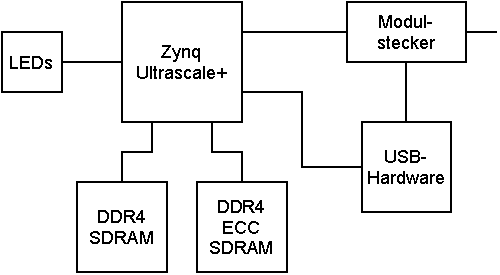
\includegraphics[width=0.7\linewidth]{bd_xu5}
    \caption{Blockdiagramm SoC Moduls XU5 von Enclustra}
    \label{fig:bd_xu5}
\end{figure}
Das Enclustra Mercury XU5 ist ein SoC Modul, auf welchem ein Xilinx Zynq Ultrascale+ ZU4EV SoC sitzt. 
Der Ultrascale ist ein System on Chip (SoC), welcher ein FPGA-System und ein ARM Prozessorsystem in einem Chip integriert. 
Das Modul hat zwei SDRAMs, wobei einer am ARM System hängt und der andere am FPGA. Beide sind über DDR4 an den SoC angeschlossen. Derjenige, welcher am ARM-System angeschlossen ist, kann mittels einem Error Correcting Code (ECC) zusätzlich noch Fehler erkennen und korrigieren. Dies brauchen wir jedoch nicht. 
Zusätzlich hat es sechs LEDs vier GPIOs und zwei Status-LEDs, welche auf die Pins \textit{PS\_ERROR} und \textit{PS\_STATUS} des SoCs geführt sind. 
Das USB 2.0 vom SoC ist per ULPI mit einem externen Chip auf dem Modul verbunden, welcher wiederum auf die Modulstecker geht. Über zwei Pins des Modulsteckers kann die Bootvariante ausgewählt werden. Somit sind mit vier verschiedenen Boot-Möglichkeiten nicht alle Möglichkeiten des SoCs vorhanden.
Das Blockschaltbild ist in Abbildung \ref{fig:bd_xu5} zu sehen. Das XU5 hat noch weitere Funktionen. 
Diese sind jedoch für dieses Projekt nicht relevant und sind daher weder auf dem Blockdiagramm noch im Text beschrieben. 
Für genauere Informationen kann die Dokumentation des Moduls angeschaut werden. \cite{xu5}

\subsubsection*{Xilinx Zynq Ultrascale+}
\begin{figure}[tb]
    \centering
    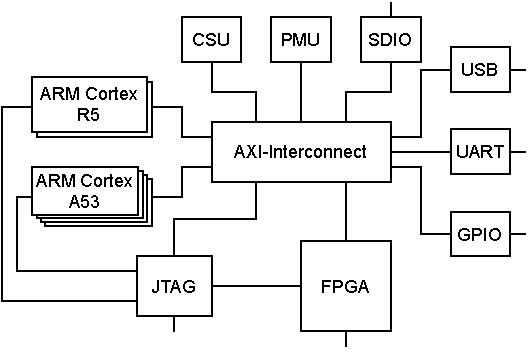
\includegraphics[width=0.8\linewidth]{bd_soc}
    \caption{Blockdiagramm des Zynq Ultrascale+ SoCs von Xilinx}
    \label{fig:bd_soc}
\end{figure}

Der Ultrascale ist ein SoC mit einem ARM Prozessorsystem und einem FPGA-System integriert in einem Chip. Das ARM-System wird auch Programmable System (PS) genannt und des FPGA-System auch Programmable Logic (PL). Das Blockschaltbild ist in Abbildung \ref{fig:bd_soc} zu sehen. Auch hier sind nur die für das Projekt relevante Blöcke abgebildet. 

Das ARM-System besteht aus zwei ARM Cortex-R5 Kernen, vier Cortex-A53 Kernen und einem Grafikkern. Der Grafikkern ist für das Projekt irrelevant und wird daher komplett verschwiegen. Zusätzlich enthält das ARM-System noch eine Configuration Security Unit (CSU) und eine Platform Management Unit (PMU). Diese beiden Blöcke sind für das Booten zuständig und während dem Betrieb für sicherheitsrelevante Funktionen, sowie dem Power Management.

Als Peripherie besitzt der SoC eine Schnittstelle für USB 3.0 und 2.0, UART, SDIO, DDR und JTAG. Zusätzlich können die GPIO Pins als Ein- oder Ausgänge verwendet werden. Die verschiedenen Prozessorkerne. die Peripherien, der Speicher und das FPGA-System sind über AXI-Interconnect-Switches zusammengeschlossen. Das JTAG ist mit drei JTAG-Controllern verbunden. Eines, welches auf das ganze System Zugriff hat, Ein zweites, welches mit dem Coresight des ARM-Systems verbunden ist. Und ein drites, welches das FPGA-System debuggen kann. Das FPGA-System ist ein Xilinx FPGA von der Ultrascale+ Familie. 

Es gibt vier Hauptdokumentationen über das SoC. Das Datenblatt\cite{datasheet}, das Technical Referenz Manual (TRM)\cite{trm}, die Software Developer Guide\cite{software} und das Packaging and Pinouts Guide\cite{packaging}.


\subsection{Entwicklungssystem}
Da das XU5 nur ein Modul ist, welches nicht selbstständig läuft, braucht es ein zusätzliches Board. Im Verlauf dieses Projektes wird dieses Board entwickelt. Damit jedoch direkt von Anfang an mit dem Entwickeln auf dem SoC begonnen werden kann, haben wir zusätzlich noch das Mercury+ PE1-200 Board von Enclustra gekauft. 

\subsubsection*{Mercury+ PE1-200 Baseboard}
\begin{figure}[tb]
    \centering
    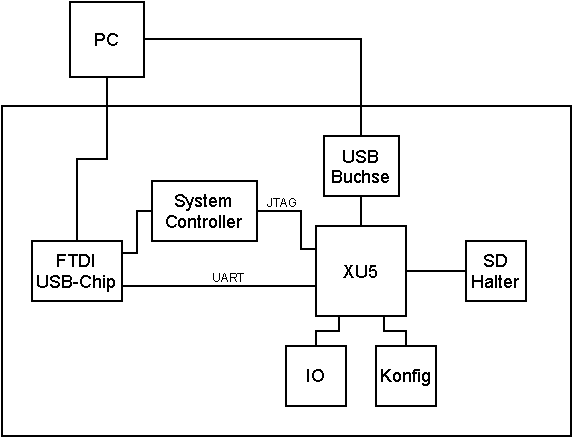
\includegraphics[width=0.7\linewidth]{bd_pe1}
    \caption{Blockdiagramm des Mercury+ PE1-200 Baseboards von Enclustra}
    \label{fig:bd_pe1}
\end{figure}
Das PE1-Board ist ein Baseboard welches alle zusätzlich notwendigen Funktionen für das XU5-Modul zur Verfügung stellt.
Das Blockdiagramm ist in Abbildung \ref{fig:bd_pe1} zu sehen. Auch hier sind wieder nur die für das Projekt relevanten Blöcke zu sehen. 
Das PE1-Board hat zwei USB Ports. Über den einen ist das JTAG und das UART geführt und den zweiten das USB Interface des SoCs. Das Routing der USB Schnittstellen kann über die Schalter auf dem Board eingestellt werden. Das JTAG wird auf einen Chip auf dem Board zu UART umgewandelt, damit mit beiden Entwicklungsumgebungen direkt ohne zusätzliche Hardware per USB auf die Debug-Schnittstelle zugegriffen werden kann. Ein von Enclustra programmierter Chip konvertiert das JTAG auf UART und ein FTDI-Chip konvertiert die beiden UART-Signale auf USB. Um zu booten wird die SD Karte gebraucht, für welche das PE1-Board eine Halterung besitzt. Zusätzlich hat das Board noch LEDs und Schalter. Die LEDs und Schalter können als IOs des SoCs gebraucht werden. Mit den Schaltern können zusätzlich Einstellungen für den Bootmodus und das Routing der USB-Pfade gesetzt werden. Um von der SD-Karte zu booten, müssen die Schalter \textit{A1} und \textit{B2} abgeschaltet sein. Um das JTAG und UART auf die Mikro-USB-Büchse zu führen, muss Schalter \textit{B2} abgeschaltet sein. Und um das USB-Interface des SoCs auf die USB-B-Buchse zu führen, muss Schalter \textit{B1} abgeschalten sein. \cite{pe1}




Das endgültigen System emuliert den Sensor der Varian vollständig. Zuerst durchläuft der Emulator die Bootsequenz des XI-Computers, damit der XI-Computer das Gefühl hat, an einem richtigen Sensor angeschlossen zu sein. Über USB kann man dann den Imager Emulator konfigurieren und die gewünschten Bilder auf den Emulator laden. Der Emulator rechnet anschliessend die Pixelfehler in die Bilder. Auf Befehl vom XI-Computer sendet der Emulator die Bilddaten, oder arbeitet einen Read- oder Write-Befehl ab. Die Pixelfehler werden nach einem vorgegebenen Muster generiert. Die Muster sollen die Zufallsverteilungen der Pixelfehler nachstellen. Da der FPGA die Pixelfehler in die Bilder einbaut, kann das gleiche Bild mit verschiedenen Pixelfehlern verwendet werden, ohne dass zusätzlich Speicherplatz benötigt wird.

\subsection{Endsystem}
\begin{figure}[b]
    \centering
    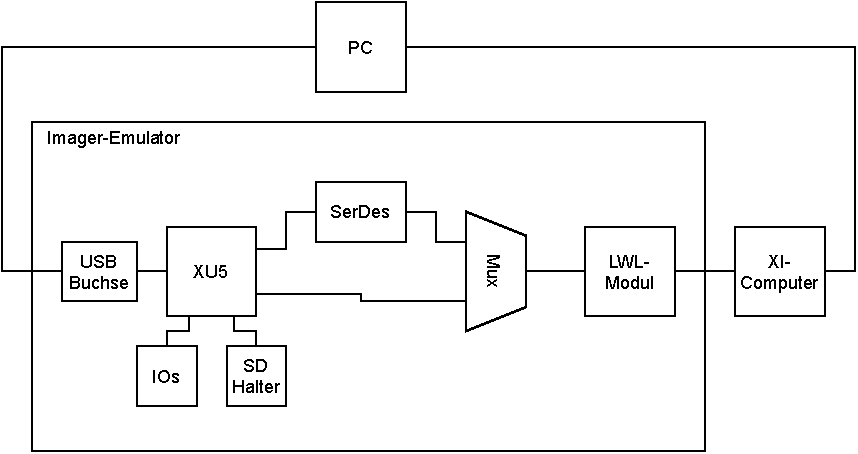
\includegraphics[width=\linewidth]{bd_top}
    \caption{Blockdiagramm des Imager-Emulators}
    \label{fig:bd_top}
\end{figure}

In Abbildung \ref{fig:bd_top} ist das Blockschaltbild des endgültigen Systems zu sehen. Das selber entwickelte Board hat einen Stecker für das XU5-Modul. Das Modul kann über den SerDes mit dem XI-Computer kommunizieren. Mit dem Mux kann zwischen dem internen und dem externen SerDes gewechselt werden. Und das SFP Modul wandelt das elektrische Signal in ein optisches um. Die Daten können über den Mikro-USB-Stecker auf den SoC geladen werden. Um zu booten hat es ein SD-Kartenhalter. Zusätzlich hat es noch LEDs und Taster, um, falls nötig, einfache Ein- und Ausgaben zu betätigen. Um zu debuggen hat es einen Stecker für die JTAG-Schnittstelle. Um diese am Computer anzuschliessen braucht es noch eine externe Hardware, welche das JTAG auf USB konvertiert. Die JTAG-Schnittstelle ist nicht auf dem Blockdiagramm, da es nur zu Debug-Zwecken dient und während des Betriebs nicht verwendet wird. 

Dieses Board ist die Arbeit des Projekt 5, welches gleichzeitig mit diesem Projekt durchgeführt wird. Für eine genauere Erklärung der Hardware und Designentscheidungen wird auf den Bericht jenes Projektes verwiesen.
